% Created by tikzDevice version 0.12 on 2019-06-14 15:08:29
% !TEX encoding = UTF-8 Unicode
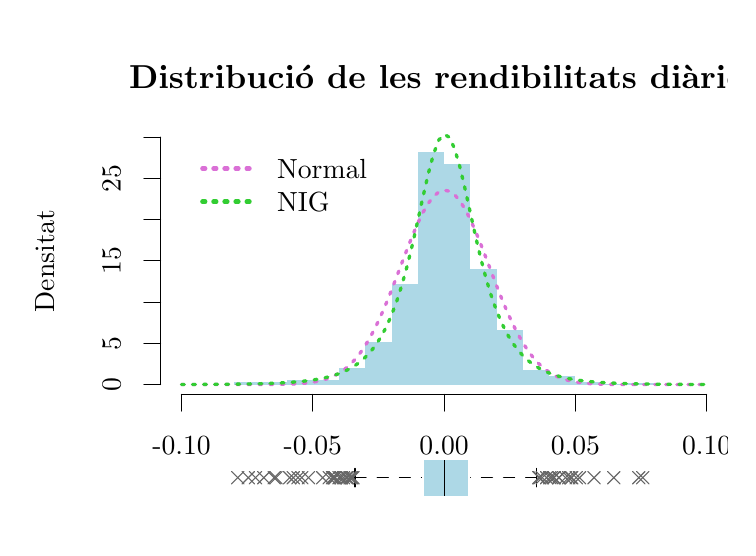
\begin{tikzpicture}[x=1pt,y=1pt]
\definecolor{fillColor}{RGB}{255,255,255}
\path[use as bounding box,fill=fillColor,fill opacity=0.00] (0,0) rectangle (252.94,180.67);
\begin{scope}
\path[clip] ( 48.00,  0.00) rectangle (252.94, 36.13);
\definecolor{fillColor}{RGB}{173,216,230}

\path[fill=fillColor] (142.84, 11.38) --
	(142.84, 24.76) --
	(159.47, 24.76) --
	(159.47, 11.38) --
	cycle;
\definecolor{drawColor}{RGB}{0,0,0}

\path[draw=drawColor,line width= 0.4pt,line join=round] (150.72, 11.38) -- (150.72, 24.76);

\path[draw=drawColor,line width= 0.4pt,dash pattern=on 4pt off 4pt ,line join=round,line cap=round] (118.29, 18.07) -- (142.84, 18.07);

\path[draw=drawColor,line width= 0.4pt,dash pattern=on 4pt off 4pt ,line join=round,line cap=round] (183.95, 18.07) -- (159.47, 18.07);

\path[draw=drawColor,line width= 0.4pt,line join=round,line cap=round] (118.29, 14.72) -- (118.29, 21.41);

\path[draw=drawColor,line width= 0.4pt,line join=round,line cap=round] (183.95, 14.72) -- (183.95, 21.41);
\definecolor{drawColor}{RGB}{255,255,255}

\path[draw=drawColor,line width= 0.4pt,line join=round,line cap=round] (142.84, 11.38) --
	(142.84, 24.76) --
	(159.47, 24.76) --
	(159.47, 11.38) --
	(142.84, 11.38);
\definecolor{drawColor}{gray}{0.40}

\path[draw=drawColor,line width= 0.4pt,line join=round,line cap=round] ( 96.77, 15.82) -- (101.27, 20.32);

\path[draw=drawColor,line width= 0.4pt,line join=round,line cap=round] ( 96.77, 20.32) -- (101.27, 15.82);

\path[draw=drawColor,line width= 0.4pt,line join=round,line cap=round] ( 77.49, 15.82) -- ( 81.99, 20.32);

\path[draw=drawColor,line width= 0.4pt,line join=round,line cap=round] ( 77.49, 20.32) -- ( 81.99, 15.82);

\path[draw=drawColor,line width= 0.4pt,line join=round,line cap=round] (183.70, 15.82) -- (188.20, 20.32);

\path[draw=drawColor,line width= 0.4pt,line join=round,line cap=round] (183.70, 20.32) -- (188.20, 15.82);

\path[draw=drawColor,line width= 0.4pt,line join=round,line cap=round] (182.43, 15.82) -- (186.93, 20.32);

\path[draw=drawColor,line width= 0.4pt,line join=round,line cap=round] (182.43, 20.32) -- (186.93, 15.82);

\path[draw=drawColor,line width= 0.4pt,line join=round,line cap=round] (113.33, 15.82) -- (117.83, 20.32);

\path[draw=drawColor,line width= 0.4pt,line join=round,line cap=round] (113.33, 20.32) -- (117.83, 15.82);

\path[draw=drawColor,line width= 0.4pt,line join=round,line cap=round] (182.82, 15.82) -- (187.32, 20.32);

\path[draw=drawColor,line width= 0.4pt,line join=round,line cap=round] (182.82, 20.32) -- (187.32, 15.82);

\path[draw=drawColor,line width= 0.4pt,line join=round,line cap=round] ( 86.81, 15.82) -- ( 91.31, 20.32);

\path[draw=drawColor,line width= 0.4pt,line join=round,line cap=round] ( 86.81, 20.32) -- ( 91.31, 15.82);

\path[draw=drawColor,line width= 0.4pt,line join=round,line cap=round] (197.19, 15.82) -- (201.69, 20.32);

\path[draw=drawColor,line width= 0.4pt,line join=round,line cap=round] (197.19, 20.32) -- (201.69, 15.82);

\path[draw=drawColor,line width= 0.4pt,line join=round,line cap=round] (104.34, 15.82) -- (108.84, 20.32);

\path[draw=drawColor,line width= 0.4pt,line join=round,line cap=round] (104.34, 20.32) -- (108.84, 15.82);

\path[draw=drawColor,line width= 0.4pt,line join=round,line cap=round] (107.87, 15.82) -- (112.37, 20.32);

\path[draw=drawColor,line width= 0.4pt,line join=round,line cap=round] (107.87, 20.32) -- (112.37, 15.82);

\path[draw=drawColor,line width= 0.4pt,line join=round,line cap=round] (193.24, 15.82) -- (197.74, 20.32);

\path[draw=drawColor,line width= 0.4pt,line join=round,line cap=round] (193.24, 20.32) -- (197.74, 15.82);

\path[draw=drawColor,line width= 0.4pt,line join=round,line cap=round] (114.98, 15.82) -- (119.48, 20.32);

\path[draw=drawColor,line width= 0.4pt,line join=round,line cap=round] (114.98, 20.32) -- (119.48, 15.82);

\path[draw=drawColor,line width= 0.4pt,line join=round,line cap=round] (110.93, 15.82) -- (115.43, 20.32);

\path[draw=drawColor,line width= 0.4pt,line join=round,line cap=round] (110.93, 20.32) -- (115.43, 15.82);

\path[draw=drawColor,line width= 0.4pt,line join=round,line cap=round] ( 99.21, 15.82) -- (103.71, 20.32);

\path[draw=drawColor,line width= 0.4pt,line join=round,line cap=round] ( 99.21, 20.32) -- (103.71, 15.82);

\path[draw=drawColor,line width= 0.4pt,line join=round,line cap=round] (192.10, 15.82) -- (196.60, 20.32);

\path[draw=drawColor,line width= 0.4pt,line join=round,line cap=round] (192.10, 20.32) -- (196.60, 15.82);

\path[draw=drawColor,line width= 0.4pt,line join=round,line cap=round] (188.04, 15.82) -- (192.54, 20.32);

\path[draw=drawColor,line width= 0.4pt,line join=round,line cap=round] (188.04, 20.32) -- (192.54, 15.82);

\path[draw=drawColor,line width= 0.4pt,line join=round,line cap=round] (187.73, 15.82) -- (192.23, 20.32);

\path[draw=drawColor,line width= 0.4pt,line join=round,line cap=round] (187.73, 20.32) -- (192.23, 15.82);

\path[draw=drawColor,line width= 0.4pt,line join=round,line cap=round] (108.84, 15.82) -- (113.34, 20.32);

\path[draw=drawColor,line width= 0.4pt,line join=round,line cap=round] (108.84, 20.32) -- (113.34, 15.82);

\path[draw=drawColor,line width= 0.4pt,line join=round,line cap=round] (185.27, 15.82) -- (189.77, 20.32);

\path[draw=drawColor,line width= 0.4pt,line join=round,line cap=round] (185.27, 20.32) -- (189.77, 15.82);

\path[draw=drawColor,line width= 0.4pt,line join=round,line cap=round] (114.25, 15.82) -- (118.75, 20.32);

\path[draw=drawColor,line width= 0.4pt,line join=round,line cap=round] (114.25, 20.32) -- (118.75, 15.82);

\path[draw=drawColor,line width= 0.4pt,line join=round,line cap=round] ( 83.08, 15.82) -- ( 87.58, 20.32);

\path[draw=drawColor,line width= 0.4pt,line join=round,line cap=round] ( 83.08, 20.32) -- ( 87.58, 15.82);

\path[draw=drawColor,line width= 0.4pt,line join=round,line cap=round] (195.96, 15.82) -- (200.46, 20.32);

\path[draw=drawColor,line width= 0.4pt,line join=round,line cap=round] (195.96, 20.32) -- (200.46, 15.82);

\path[draw=drawColor,line width= 0.4pt,line join=round,line cap=round] (189.77, 15.82) -- (194.27, 20.32);

\path[draw=drawColor,line width= 0.4pt,line join=round,line cap=round] (189.77, 20.32) -- (194.27, 15.82);

\path[draw=drawColor,line width= 0.4pt,line join=round,line cap=round] (218.60, 15.82) -- (223.10, 20.32);

\path[draw=drawColor,line width= 0.4pt,line join=round,line cap=round] (218.60, 20.32) -- (223.10, 15.82);

\path[draw=drawColor,line width= 0.4pt,line join=round,line cap=round] (106.71, 15.82) -- (111.21, 20.32);

\path[draw=drawColor,line width= 0.4pt,line join=round,line cap=round] (106.71, 20.32) -- (111.21, 15.82);

\path[draw=drawColor,line width= 0.4pt,line join=round,line cap=round] (220.02, 15.82) -- (224.52, 20.32);

\path[draw=drawColor,line width= 0.4pt,line join=round,line cap=round] (220.02, 20.32) -- (224.52, 15.82);

\path[draw=drawColor,line width= 0.4pt,line join=round,line cap=round] (202.43, 15.82) -- (206.93, 20.32);

\path[draw=drawColor,line width= 0.4pt,line join=round,line cap=round] (202.43, 20.32) -- (206.93, 15.82);

\path[draw=drawColor,line width= 0.4pt,line join=round,line cap=round] (194.35, 15.82) -- (198.85, 20.32);

\path[draw=drawColor,line width= 0.4pt,line join=round,line cap=round] (194.35, 20.32) -- (198.85, 15.82);

\path[draw=drawColor,line width= 0.4pt,line join=round,line cap=round] (108.80, 15.82) -- (113.30, 20.32);

\path[draw=drawColor,line width= 0.4pt,line join=round,line cap=round] (108.80, 20.32) -- (113.30, 15.82);

\path[draw=drawColor,line width= 0.4pt,line join=round,line cap=round] ( 95.45, 15.82) -- ( 99.95, 20.32);

\path[draw=drawColor,line width= 0.4pt,line join=round,line cap=round] ( 95.45, 20.32) -- ( 99.95, 15.82);

\path[draw=drawColor,line width= 0.4pt,line join=round,line cap=round] (108.39, 15.82) -- (112.89, 20.32);

\path[draw=drawColor,line width= 0.4pt,line join=round,line cap=round] (108.39, 20.32) -- (112.89, 15.82);

\path[draw=drawColor,line width= 0.4pt,line join=round,line cap=round] ( 92.41, 15.82) -- ( 96.91, 20.32);

\path[draw=drawColor,line width= 0.4pt,line join=round,line cap=round] ( 92.41, 20.32) -- ( 96.91, 15.82);

\path[draw=drawColor,line width= 0.4pt,line join=round,line cap=round] (114.71, 15.82) -- (119.21, 20.32);

\path[draw=drawColor,line width= 0.4pt,line join=round,line cap=round] (114.71, 20.32) -- (119.21, 15.82);

\path[draw=drawColor,line width= 0.4pt,line join=round,line cap=round] ( 87.48, 15.82) -- ( 91.98, 20.32);

\path[draw=drawColor,line width= 0.4pt,line join=round,line cap=round] ( 87.48, 20.32) -- ( 91.98, 15.82);

\path[draw=drawColor,line width= 0.4pt,line join=round,line cap=round] (113.25, 15.82) -- (117.75, 20.32);

\path[draw=drawColor,line width= 0.4pt,line join=round,line cap=round] (113.25, 20.32) -- (117.75, 15.82);

\path[draw=drawColor,line width= 0.4pt,line join=round,line cap=round] (186.40, 15.82) -- (190.90, 20.32);

\path[draw=drawColor,line width= 0.4pt,line join=round,line cap=round] (186.40, 20.32) -- (190.90, 15.82);

\path[draw=drawColor,line width= 0.4pt,line join=round,line cap=round] (112.87, 15.82) -- (117.37, 20.32);

\path[draw=drawColor,line width= 0.4pt,line join=round,line cap=round] (112.87, 20.32) -- (117.37, 15.82);

\path[draw=drawColor,line width= 0.4pt,line join=round,line cap=round] (111.06, 15.82) -- (115.56, 20.32);

\path[draw=drawColor,line width= 0.4pt,line join=round,line cap=round] (111.06, 20.32) -- (115.56, 15.82);

\path[draw=drawColor,line width= 0.4pt,line join=round,line cap=round] (110.28, 15.82) -- (114.78, 20.32);

\path[draw=drawColor,line width= 0.4pt,line join=round,line cap=round] (110.28, 20.32) -- (114.78, 15.82);

\path[draw=drawColor,line width= 0.4pt,line join=round,line cap=round] ( 73.64, 15.82) -- ( 78.14, 20.32);

\path[draw=drawColor,line width= 0.4pt,line join=round,line cap=round] ( 73.64, 20.32) -- ( 78.14, 15.82);

\path[draw=drawColor,line width= 0.4pt,line join=round,line cap=round] ( 93.74, 15.82) -- ( 98.24, 20.32);

\path[draw=drawColor,line width= 0.4pt,line join=round,line cap=round] ( 93.74, 20.32) -- ( 98.24, 15.82);

\path[draw=drawColor,line width= 0.4pt,line join=round,line cap=round] (189.64, 15.82) -- (194.14, 20.32);

\path[draw=drawColor,line width= 0.4pt,line join=round,line cap=round] (189.64, 20.32) -- (194.14, 15.82);

\path[draw=drawColor,line width= 0.4pt,line join=round,line cap=round] (115.31, 15.82) -- (119.81, 20.32);

\path[draw=drawColor,line width= 0.4pt,line join=round,line cap=round] (115.31, 20.32) -- (119.81, 15.82);

\path[draw=drawColor,line width= 0.4pt,line join=round,line cap=round] (194.08, 15.82) -- (198.58, 20.32);

\path[draw=drawColor,line width= 0.4pt,line join=round,line cap=round] (194.08, 20.32) -- (198.58, 15.82);

\path[draw=drawColor,line width= 0.4pt,line join=round,line cap=round] (187.05, 15.82) -- (191.55, 20.32);

\path[draw=drawColor,line width= 0.4pt,line join=round,line cap=round] (187.05, 20.32) -- (191.55, 15.82);

\path[draw=drawColor,line width= 0.4pt,line join=round,line cap=round] ( 80.07, 15.82) -- ( 84.57, 20.32);

\path[draw=drawColor,line width= 0.4pt,line join=round,line cap=round] ( 80.07, 20.32) -- ( 84.57, 15.82);

\path[draw=drawColor,line width= 0.4pt,line join=round,line cap=round] (111.91, 15.82) -- (116.41, 20.32);

\path[draw=drawColor,line width= 0.4pt,line join=round,line cap=round] (111.91, 20.32) -- (116.41, 15.82);

\path[draw=drawColor,line width= 0.4pt,line join=round,line cap=round] (209.56, 15.82) -- (214.06, 20.32);

\path[draw=drawColor,line width= 0.4pt,line join=round,line cap=round] (209.56, 20.32) -- (214.06, 15.82);
\end{scope}
\begin{scope}
\path[clip] (  0.00, 36.13) rectangle (252.94,180.67);
\definecolor{drawColor}{RGB}{0,0,0}

\node[text=drawColor,anchor=base,inner sep=0pt, outer sep=0pt, scale=  1.20] at (150.47,158.53) {\bfseries Distribució de les rendibilitats diàries};

\node[text=drawColor,rotate= 90.00,anchor=base,inner sep=0pt, outer sep=0pt, scale=  1.00] at (  9.60, 96.40) {Densitat};
\end{scope}
\begin{scope}
\path[clip] (  0.00,  0.00) rectangle (252.94,180.67);
\definecolor{drawColor}{RGB}{0,0,0}

\path[draw=drawColor,line width= 0.4pt,line join=round,line cap=round] ( 55.59, 48.13) -- (245.35, 48.13);

\path[draw=drawColor,line width= 0.4pt,line join=round,line cap=round] ( 55.59, 48.13) -- ( 55.59, 42.13);

\path[draw=drawColor,line width= 0.4pt,line join=round,line cap=round] (103.03, 48.13) -- (103.03, 42.13);

\path[draw=drawColor,line width= 0.4pt,line join=round,line cap=round] (150.47, 48.13) -- (150.47, 42.13);

\path[draw=drawColor,line width= 0.4pt,line join=round,line cap=round] (197.91, 48.13) -- (197.91, 42.13);

\path[draw=drawColor,line width= 0.4pt,line join=round,line cap=round] (245.35, 48.13) -- (245.35, 42.13);

\node[text=drawColor,anchor=base,inner sep=0pt, outer sep=0pt, scale=  1.00] at ( 55.59, 26.53) {-0.10};

\node[text=drawColor,anchor=base,inner sep=0pt, outer sep=0pt, scale=  1.00] at (103.03, 26.53) {-0.05};

\node[text=drawColor,anchor=base,inner sep=0pt, outer sep=0pt, scale=  1.00] at (150.47, 26.53) {0.00};

\node[text=drawColor,anchor=base,inner sep=0pt, outer sep=0pt, scale=  1.00] at (197.91, 26.53) {0.05};

\node[text=drawColor,anchor=base,inner sep=0pt, outer sep=0pt, scale=  1.00] at (245.35, 26.53) {0.10};

\path[draw=drawColor,line width= 0.4pt,line join=round,line cap=round] ( 48.00, 51.71) -- ( 48.00,141.10);

\path[draw=drawColor,line width= 0.4pt,line join=round,line cap=round] ( 48.00, 51.71) -- ( 42.00, 51.71);

\path[draw=drawColor,line width= 0.4pt,line join=round,line cap=round] ( 48.00, 66.61) -- ( 42.00, 66.61);

\path[draw=drawColor,line width= 0.4pt,line join=round,line cap=round] ( 48.00, 81.51) -- ( 42.00, 81.51);

\path[draw=drawColor,line width= 0.4pt,line join=round,line cap=round] ( 48.00, 96.40) -- ( 42.00, 96.40);

\path[draw=drawColor,line width= 0.4pt,line join=round,line cap=round] ( 48.00,111.30) -- ( 42.00,111.30);

\path[draw=drawColor,line width= 0.4pt,line join=round,line cap=round] ( 48.00,126.20) -- ( 42.00,126.20);

\path[draw=drawColor,line width= 0.4pt,line join=round,line cap=round] ( 48.00,141.10) -- ( 42.00,141.10);

\node[text=drawColor,rotate= 90.00,anchor=base,inner sep=0pt, outer sep=0pt, scale=  1.00] at ( 33.60, 51.71) {0};

\node[text=drawColor,rotate= 90.00,anchor=base,inner sep=0pt, outer sep=0pt, scale=  1.00] at ( 33.60, 66.61) {5};

\node[text=drawColor,rotate= 90.00,anchor=base,inner sep=0pt, outer sep=0pt, scale=  1.00] at ( 33.60, 96.40) {15};

\node[text=drawColor,rotate= 90.00,anchor=base,inner sep=0pt, outer sep=0pt, scale=  1.00] at ( 33.60,126.20) {25};
\end{scope}
\begin{scope}
\path[clip] ( 48.00, 48.13) rectangle (252.94,144.67);
\definecolor{fillColor}{RGB}{173,216,230}

\path[fill=fillColor] ( 74.57, 51.71) rectangle ( 84.06, 52.60);

\path[fill=fillColor] ( 84.06, 51.71) rectangle ( 93.54, 52.60);

\path[fill=fillColor] ( 93.54, 51.71) rectangle (103.03, 53.19);

\path[fill=fillColor] (103.03, 51.71) rectangle (112.52, 53.49);

\path[fill=fillColor] (112.52, 51.71) rectangle (122.01, 57.65);

\path[fill=fillColor] (122.01, 51.71) rectangle (131.50, 67.14);

\path[fill=fillColor] (131.50, 51.71) rectangle (140.98, 88.21);

\path[fill=fillColor] (140.98, 51.71) rectangle (150.47,135.70);

\path[fill=fillColor] (150.47, 51.71) rectangle (159.96,131.25);

\path[fill=fillColor] (159.96, 51.71) rectangle (169.45, 93.56);

\path[fill=fillColor] (169.45, 51.71) rectangle (178.94, 71.30);

\path[fill=fillColor] (178.94, 51.71) rectangle (188.43, 57.05);

\path[fill=fillColor] (188.43, 51.71) rectangle (197.91, 54.68);

\path[fill=fillColor] (197.91, 51.71) rectangle (207.40, 52.60);

\path[fill=fillColor] (207.40, 51.71) rectangle (216.89, 52.01);

\path[fill=fillColor] (216.89, 51.71) rectangle (226.38, 52.30);
\definecolor{drawColor}{RGB}{218,112,214}

\path[draw=drawColor,line width= 1.2pt,dash pattern=on 1pt off 3pt ,line join=round,line cap=round] ( 55.59, 51.71) --
	( 57.49, 51.71) --
	( 59.39, 51.71) --
	( 61.28, 51.71) --
	( 63.18, 51.71) --
	( 65.08, 51.71) --
	( 66.98, 51.71) --
	( 68.87, 51.71) --
	( 70.77, 51.71) --
	( 72.67, 51.71) --
	( 74.57, 51.71) --
	( 76.46, 51.71) --
	( 78.36, 51.71) --
	( 80.26, 51.72) --
	( 82.16, 51.72) --
	( 84.06, 51.72) --
	( 85.95, 51.73) --
	( 87.85, 51.74) --
	( 89.75, 51.76) --
	( 91.65, 51.79) --
	( 93.54, 51.83) --
	( 95.44, 51.90) --
	( 97.34, 51.99) --
	( 99.24, 52.12) --
	(101.13, 52.30) --
	(103.03, 52.56) --
	(104.93, 52.91) --
	(106.83, 53.37) --
	(108.72, 53.99) --
	(110.62, 54.80) --
	(112.52, 55.83) --
	(114.42, 57.13) --
	(116.31, 58.74) --
	(118.21, 60.71) --
	(120.11, 63.06) --
	(122.01, 65.84) --
	(123.91, 69.05) --
	(125.80, 72.69) --
	(127.70, 76.74) --
	(129.60, 81.17) --
	(131.50, 85.89) --
	(133.39, 90.83) --
	(135.29, 95.85) --
	(137.19,100.83) --
	(139.09,105.62) --
	(140.98,110.05) --
	(142.88,113.97) --
	(144.78,117.23) --
	(146.68,119.70) --
	(148.57,121.29) --
	(150.47,121.93) --
	(152.37,121.60) --
	(154.27,120.30) --
	(156.17,118.09) --
	(158.06,115.06) --
	(159.96,111.33) --
	(161.86,107.04) --
	(163.76,102.35) --
	(165.65, 97.42) --
	(167.55, 92.39) --
	(169.45, 87.41) --
	(171.35, 82.61) --
	(173.24, 78.08) --
	(175.14, 73.91) --
	(177.04, 70.13) --
	(178.94, 66.79) --
	(180.83, 63.88) --
	(182.73, 61.40) --
	(184.63, 59.31) --
	(186.53, 57.60) --
	(188.43, 56.20) --
	(190.32, 55.09) --
	(192.22, 54.22) --
	(194.12, 53.55) --
	(196.02, 53.04) --
	(197.91, 52.65) --
	(199.81, 52.37) --
	(201.71, 52.17) --
	(203.61, 52.02) --
	(205.50, 51.92) --
	(207.40, 51.85) --
	(209.30, 51.80) --
	(211.20, 51.77) --
	(213.09, 51.75) --
	(214.99, 51.73) --
	(216.89, 51.73) --
	(218.79, 51.72) --
	(220.69, 51.72) --
	(222.58, 51.71) --
	(224.48, 51.71) --
	(226.38, 51.71) --
	(228.28, 51.71) --
	(230.17, 51.71) --
	(232.07, 51.71) --
	(233.97, 51.71) --
	(235.87, 51.71) --
	(237.76, 51.71) --
	(239.66, 51.71) --
	(241.56, 51.71) --
	(243.46, 51.71) --
	(245.35, 51.71);
\definecolor{drawColor}{RGB}{50,205,50}

\path[draw=drawColor,line width= 1.2pt,dash pattern=on 1pt off 3pt ,line join=round,line cap=round] ( 55.59, 51.74) --
	( 57.49, 51.75) --
	( 59.39, 51.75) --
	( 61.28, 51.76) --
	( 63.18, 51.77) --
	( 65.08, 51.78) --
	( 66.98, 51.79) --
	( 68.87, 51.80) --
	( 70.77, 51.81) --
	( 72.67, 51.83) --
	( 74.57, 51.85) --
	( 76.46, 51.88) --
	( 78.36, 51.90) --
	( 80.26, 51.94) --
	( 82.16, 51.98) --
	( 84.06, 52.02) --
	( 85.95, 52.08) --
	( 87.85, 52.14) --
	( 89.75, 52.22) --
	( 91.65, 52.31) --
	( 93.54, 52.42) --
	( 95.44, 52.55) --
	( 97.34, 52.70) --
	( 99.24, 52.88) --
	(101.13, 53.10) --
	(103.03, 53.36) --
	(104.93, 53.67) --
	(106.83, 54.04) --
	(108.72, 54.48) --
	(110.62, 55.02) --
	(112.52, 55.66) --
	(114.42, 56.44) --
	(116.31, 57.38) --
	(118.21, 58.52) --
	(120.11, 59.90) --
	(122.01, 61.57) --
	(123.91, 63.59) --
	(125.80, 66.04) --
	(127.70, 69.00) --
	(129.60, 72.57) --
	(131.50, 76.85) --
	(133.39, 81.94) --
	(135.29, 87.91) --
	(137.19, 94.81) --
	(139.09,102.58) --
	(140.98,111.01) --
	(142.88,119.70) --
	(144.78,128.01) --
	(146.68,135.10) --
	(148.57,140.07) --
	(150.47,142.17) --
	(152.37,141.06) --
	(154.27,136.92) --
	(156.17,130.39) --
	(158.06,122.36) --
	(159.96,113.71) --
	(161.86,105.15) --
	(163.76, 97.15) --
	(165.65, 89.96) --
	(167.55, 83.70) --
	(169.45, 78.34) --
	(171.35, 73.82) --
	(173.24, 70.04) --
	(175.14, 66.90) --
	(177.04, 64.30) --
	(178.94, 62.16) --
	(180.83, 60.38) --
	(182.73, 58.92) --
	(184.63, 57.71) --
	(186.53, 56.72) --
	(188.43, 55.89) --
	(190.32, 55.21) --
	(192.22, 54.64) --
	(194.12, 54.17) --
	(196.02, 53.77) --
	(197.91, 53.45) --
	(199.81, 53.17) --
	(201.71, 52.94) --
	(203.61, 52.75) --
	(205.50, 52.59) --
	(207.40, 52.46) --
	(209.30, 52.34) --
	(211.20, 52.25) --
	(213.09, 52.17) --
	(214.99, 52.10) --
	(216.89, 52.04) --
	(218.79, 51.99) --
	(220.69, 51.95) --
	(222.58, 51.91) --
	(224.48, 51.88) --
	(226.38, 51.86) --
	(228.28, 51.84) --
	(230.17, 51.82) --
	(232.07, 51.80) --
	(233.97, 51.79) --
	(235.87, 51.78) --
	(237.76, 51.77) --
	(239.66, 51.76) --
	(241.56, 51.75) --
	(243.46, 51.75) --
	(245.35, 51.74);

\path[] ( 54.15,141.78) rectangle (127.17,105.78);
\definecolor{drawColor}{RGB}{218,112,214}

\path[draw=drawColor,line width= 1.6pt,dash pattern=on 1pt off 3pt ,line join=round,line cap=round] ( 63.15,129.78) -- ( 81.15,129.78);
\definecolor{drawColor}{RGB}{50,205,50}

\path[draw=drawColor,line width= 1.6pt,dash pattern=on 1pt off 3pt ,line join=round,line cap=round] ( 63.15,117.78) -- ( 81.15,117.78);
\definecolor{drawColor}{RGB}{0,0,0}

\node[text=drawColor,anchor=base west,inner sep=0pt, outer sep=0pt, scale=  1.00] at ( 90.15,126.34) {Normal};

\node[text=drawColor,anchor=base west,inner sep=0pt, outer sep=0pt, scale=  1.00] at ( 90.15,114.34) {NIG};
\end{scope}
\end{tikzpicture}
